\documentclass{article}
\usepackage{amsmath}
\usepackage{graphicx}
\usepackage{subcaption}
\usepackage[utf8]{inputenc}

\title{Advanced Algorithms Project Report}
\author{Guglielmo Manneschi, Andrea Mecchia}
\date{July 2019}

\begin{document}

\maketitle

\section{Introduction}
Pattern-matching algorithms are a class of string algorithms that deals with searching an occurrence of a pattern inside a larger string.

These methods can not only be used with character strings, e.g. search a word inside an English text, but also with every other type of sequences of symbols, such as binary strings or DNA sequences. The size of these strings may be so large that efficient algorithms are needed to make the problem tractable, since the naive approach has a time complexity of $\mathcal{O}(NM)$

In the next sections we will describe three different algorithms, for each one we will give a brief description of the main ideas behind that algorithm, specify its spatial and time complexities, evaluate its performance on random strings for different text and pattern lengths.

\section{Boyer-Moore algorithm}

\subsection{Description}
The basic idea of the Boyer-Moore algorithm is that more information can be gained by matching the pattern from right to left. Additionally some observations allows to skip more than one character in the search process when the relative conditions are met, so that the number of characters processed in the text can become, and usually become in practice, smaller than its size.

A first observation is that if the current character is not known to occur in the pattern, we can shift the index by the size of the pattern. Moreover, if the character occurs at his rightmost position at $i$ characters from the end, the index can be shifted by $i$. If none of these conditions are met, we should start shifting the index to the left to compare if the rest of the pattern is matched.

At this point it can happen that the pattern is matched, and conclude the procedure, or we may find a mismatch. In the latter case there are two additional performance improvements that we can take into account. The first is based on the same reasoning explained before, and allows to slide the index so to match the character with the position of the last occurrence in the pattern. The second one is a bit more sophisticated and it allows to shift the index to match the rightmost reoccurrence in the pattern of the just analyzed substring.

\subsection{Implementation and performance evaluation}

For the implementation of the algorithm two additional arrays are needed. The first one to store the information required to apply the first observations, and it has the size of the alphabet. The second one for the last observation, with the size of the pattern. Hence the algorithm requires a dynamic memory allocation of $\mathcal{O}(|M|+|\Sigma|)$, with $|M|$ the pattern length and $|\Sigma|$ the cardinality of the alphabet.

The time complexity of the preprocessing part in which the two arrays are built is not analyzed since for patterns that are much shorter than the text is negligible.

\begin{figure}
  \centering
  \begin{subfigure}[b]{0.4\linewidth}
    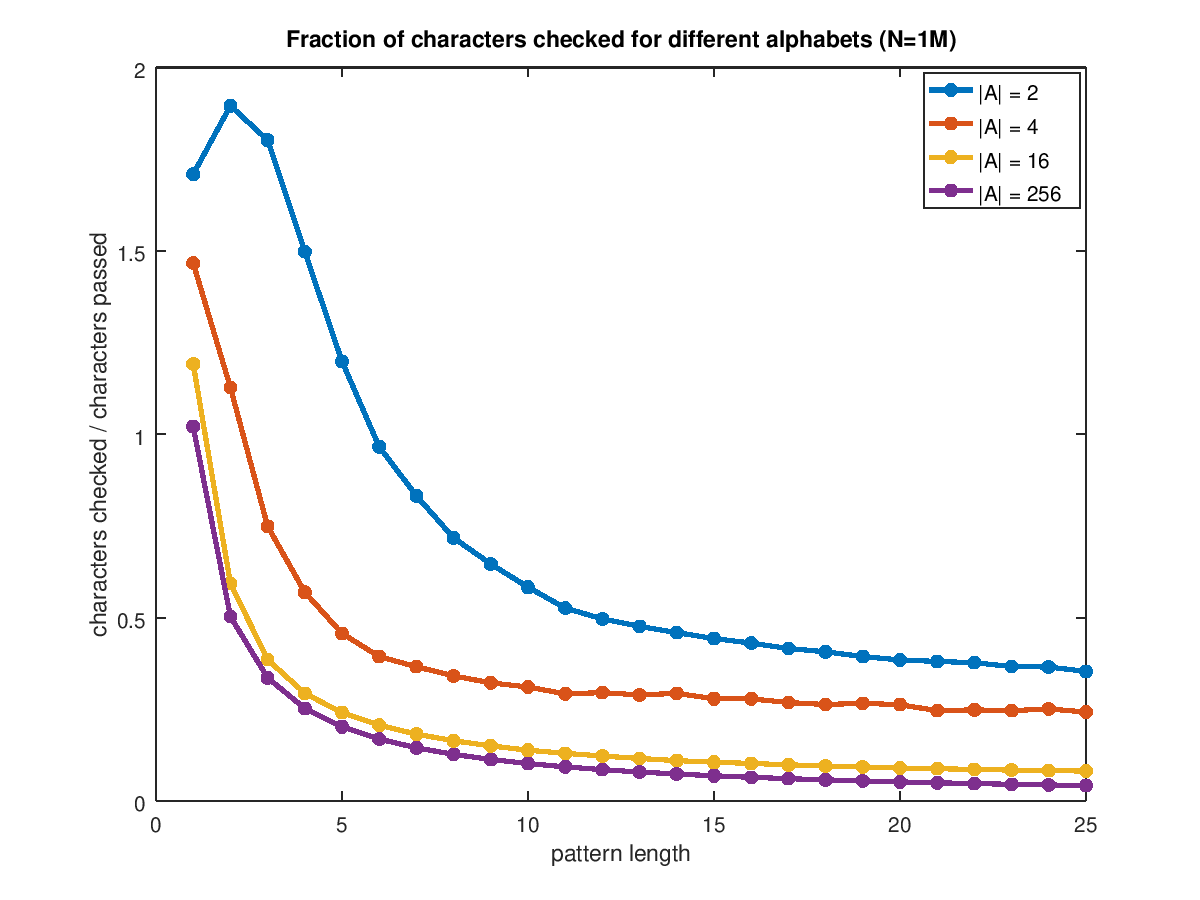
\includegraphics[width=\linewidth]{boyer3.png}
     \caption{Fraction of characters checked over characters passed in text.}
  \end{subfigure}
  \begin{subfigure}[b]{0.4\linewidth}
    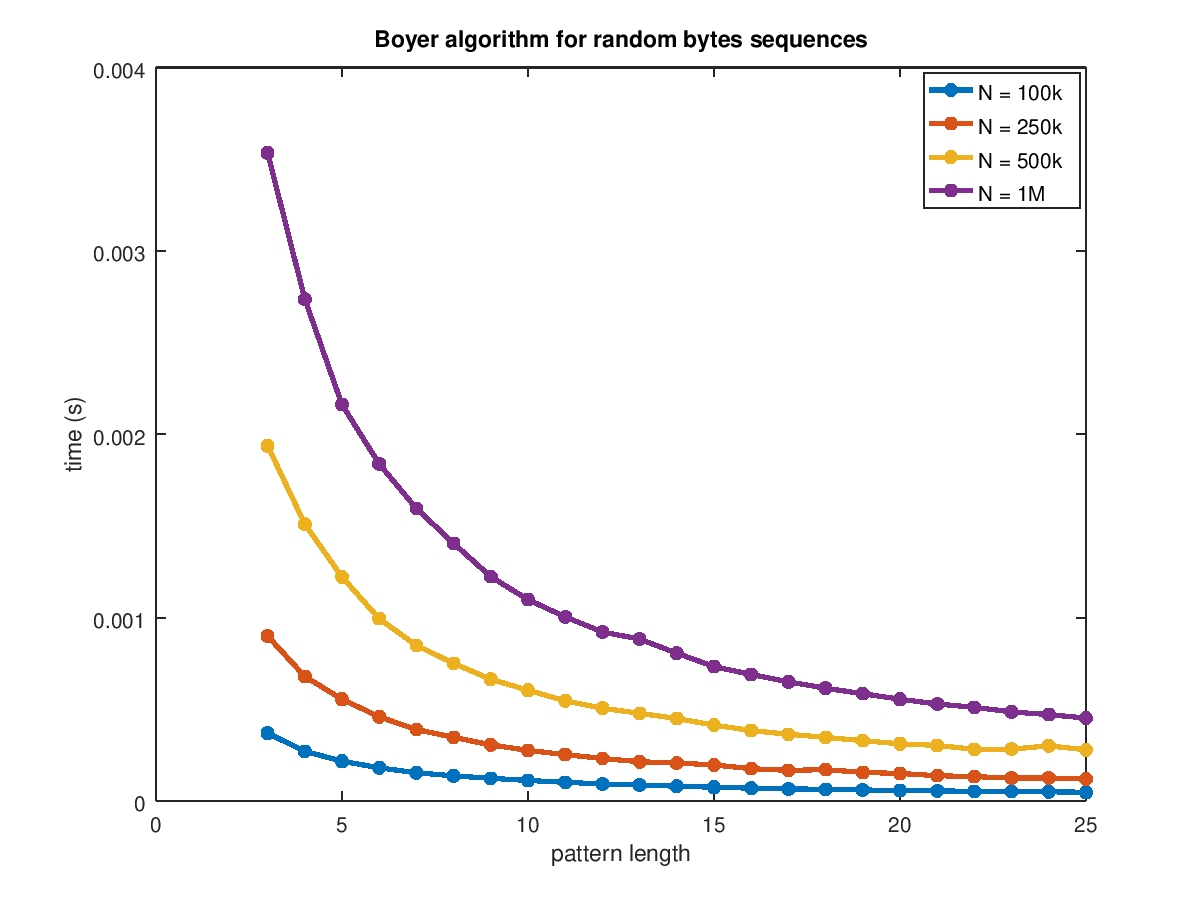
\includegraphics[width=\linewidth]{boyer1.png}
    \caption{Average time comparison for different text and pattern lengths.}
  \end{subfigure}
  \begin{subfigure}[b]{0.5\linewidth}
    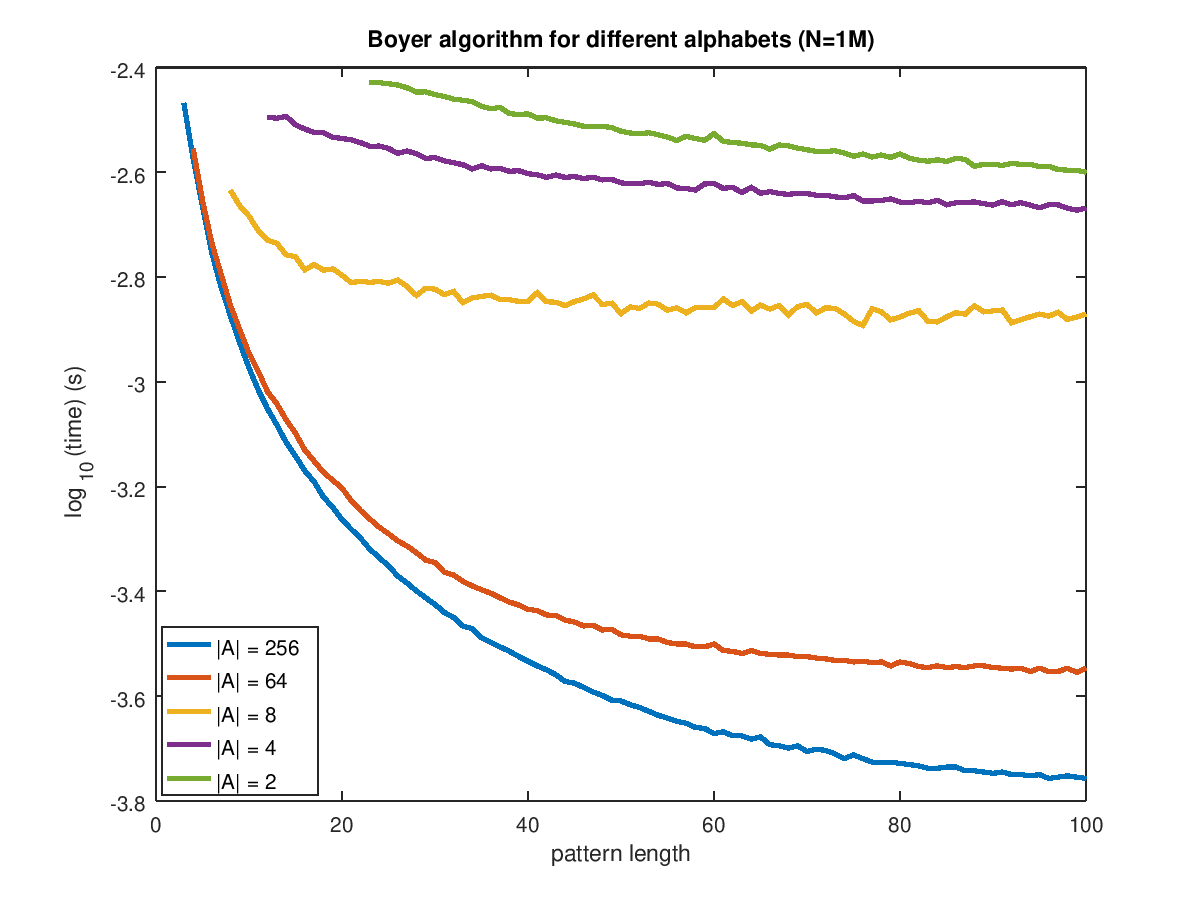
\includegraphics[width=\linewidth]{boyer2.png}
    \caption{Average time comparison for different alphabet sizes.}
  \end{subfigure}
  \caption{Boyer-Moore algorithm experiments.}
  \label{fig:boyer}
\end{figure}

The authors of the algorithm claims that the search part is ``usually sublinear'', in the sense that the number of characters of the text inspected is usually less than the number of characters passed. This behaviour is even more frequent when the length of the pattern increases. To verify this result we measured the average fraction of characters checked over characters passed (in the text string) for random strings and showed the result in Figure~\ref{fig:boyer}a. As we expected, this fraction is usually below $1$ and decreases with the length of the pattern and the size of the alphabet.

We also made a performance comparison of the complete algorithm (including the preprocessing time) to verify that the real elapsed time reflects this behaviour. In Figure~\ref{fig:boyer}b we can see how the performances increase proportionally to the pattern length, for different lengths of the text. It is interesting to note that the preprocessing of the pattern doesn't affect the performances, since its size is negligible with respect to the one of the text.

In Figure~\ref{fig:boyer}c we can see how the performances increase with the pattern lengths for different alphabet's sizes. We can see that for binary strings and for 4 characters alphabets (such as DNA sequences) the speedup is not very high, while is more evident when the alphabet sizes is high, such as 64 (English lowercase, uppercase and some punctuation characters) and 256 (bytes).

This difference in speedups is due to the fact that the first observation allows to shift the current position of the distance from the rightmost occurrence of a character to the end of the pattern. For small alphabet sizes and random strings the average distance of any characters is of course smaller than the case of greater alphabets, hence with smaller ones these shifts are of smaller size.

\section{Karp-Rabin algorithm}

\subsection{Description}
The Karp-Rabin algorithm is a probabilistic algorithm (with two deterministic variants). The fundamental idea of the Karp-Rabin algorithm is to apply an injective function to a string, similar to a cryptographic hash function, to obtain a compressed representation of the string itself, called fingerprint, which is easier to compare.

The fingerprint function associates a unique fingerprint $f(c)$ to each character $c \in \sum$. The application of the fingerprint function to a sequence of characters $s = \{c \mid c \in \sum\}^*$ is given by the composition of the fingerprints of the single characters by means of some operator $*$:

\begin{equation*} \notag
    f(s) = f(s[0]) * f(s[1]) * f(s[2]) ... f(s[n - 1]) * f(s[n])
\end{equation*}

The fingerprint injective function is such that it is possible to define the inverse element $g = f^{-1} \mid g * f = 1 \forall c \in \sum$ where $1$ is the neutral element of the fingerprint set w.r.t. the operation $*$.

These properties allow to efficiently compute the fingerprint of substring $s[n ... m]$ starting from the substring $f(s[n - 1 ... m - 1])$:

\begin{equation} \notag
\begin{split}
f(s[n ... m]) &= f^{-1}(s[n - 1]) * f(s[n - 1 ... m - 1]) * f(s[m]) \\
    &= f^{-1}(s[n - 1]) * f(s[n - 1]) ... f(s[m - 1]) * f(s[m]) \\
    &= 1 * f(s[n]) * f(s[n + 1]) ... f(s[m - 1]) * f(s[m]) \\
    &= 1 * f(s[n ... m])
\end{split}
\end{equation}

The fingerprint function is injective, thus $s = r \implies f(s) = f(r)$ and $f(s) \ne f(r) \implies s \ne r$. However it is true that $\exists s, r, s \ne r \mid f(r) = f(s)$, in which case a false match is generated. The probability of a false match depends on the particular family of fingerprint functions employed. In order to reduce the probability of a false match we can always employ multiple fingerprints of the same family chosen at random (i.e. independently). Being $k$ the number of independent fingerprints and $p_i$ the probability of a false match generated by fingerprint $f_i, 0 \le i < k$ the probability of correctly matching the pattern in the text is $1 - \prod_{i = 0}^k p_i$.

This approach yields linear time complexity $\mathcal{O}(n + m), n = |text|, m = |pattern|$ and a space complexity proportional to the size of the alphabet set $\mathcal{O}(|\sum|)$.

\subsection{Implementation}
We applied the Karp-Rabin algorithm to the classical problem of pattern matching. The alphabet size is $2^{sizeof(char)} = 2^8 = 256$. The pattern length is $m$ and the text length is $n \ge m$.

The adopted family of fingerprint functions maps each character to a unique element of the group $(M_p, \cdot)$, where $M_p$ is a $2 \times 2$ matrix over the set $Z_p$, $1 <= p <= n m^2$ is a prime number and the operation $\cdot$ is the matrix dot product $\mod p$. The inverse element $g = f^{-1}$ is trivially the inverse matrix $M^{-1}$. The prime $p$ can be chosen randomly by testing random numbers for primality without loss of efficiency, provided that an efficient primality test algorithm is employed (e.g. Miller-Rabin primality test).

We build the map of fingerprints $\{f_k(c) \mid c \in \sum\}$ and inverse fingerprints $\{f_k^{-1}(c) \mid c \in \sum\}$ for each fingerprint function $f_k$ starting from the binary representation of $c$ and from the binary fingerprints $f_k(d), f_k^{-1}(d), d = \{0, 1\}$. Note that this computation can be done offline assuming some appropriate values for $p_k$.

Then we compute the fingerprint of the pattern string $f_k(s_p)$ and the fingerprint of the text substring $f_k(s_t[0 ... n])$ for each fingerprint function $k$. Using the aforementioned properties we can then easily compute $f_k(s_t[i ... i + n]), i + n < m$ iteratively.

If $\exists i \mid \forall k f_k(s_p) = f_k(s_t[i ... i + n])$ the pattern is matched with probability $1 - p^k$, otherwise the pattern has no match in the string $s_t$. The probability of generating a false match employing a single fingerprint of this family is $\le \frac{6.971}{m}$.

The adopted family of fingerprint function has an elegant update method (multiply by the inverse matrix) but it is not very efficient; each update requires two modular matrix dot product which are very expensive.

\subsection{Performance evaluation}

\begin{figure}
  \centering
  \begin{subfigure}[b]{0.4\linewidth}
    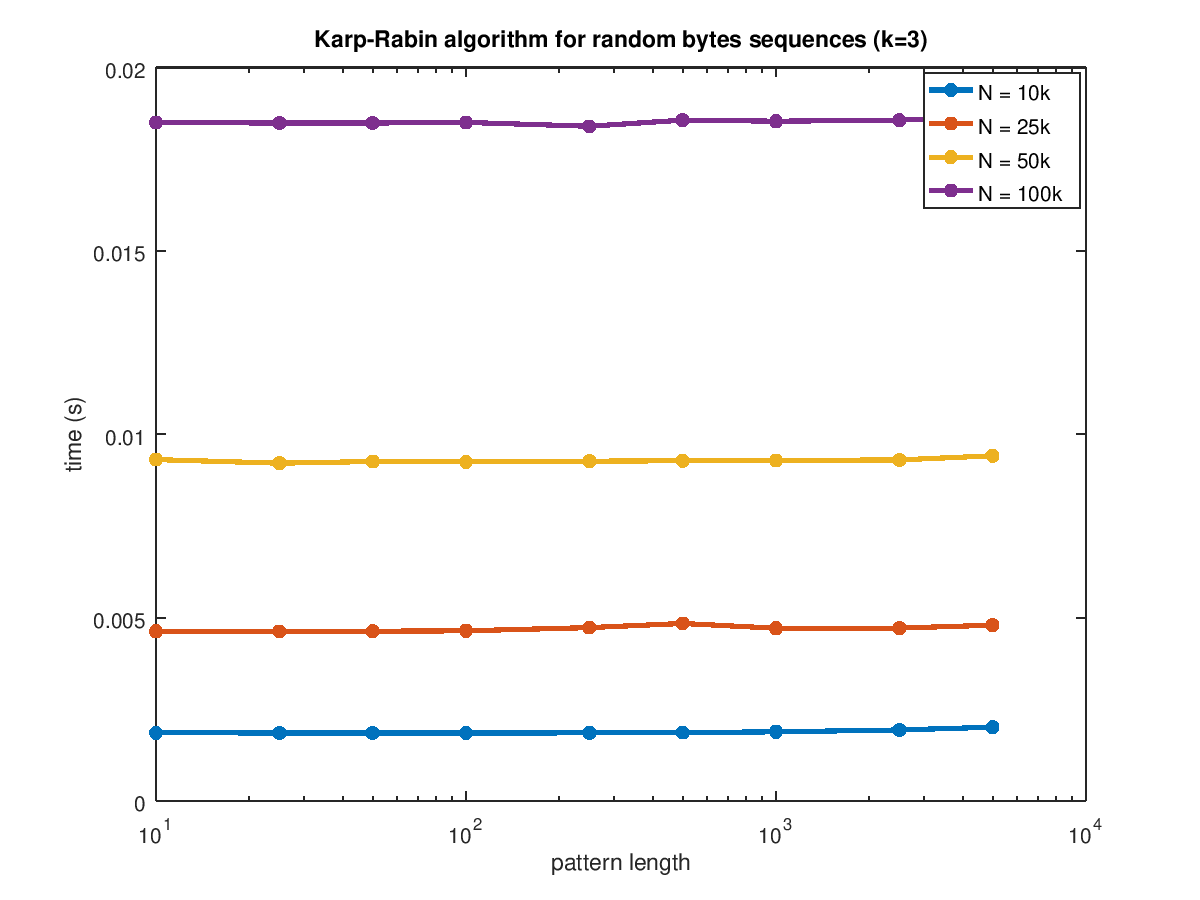
\includegraphics[width=\linewidth]{karp1.png}
     \caption{Average time comparison for different text and pattern lengths.}
  \end{subfigure}
  \begin{subfigure}[b]{0.4\linewidth}
    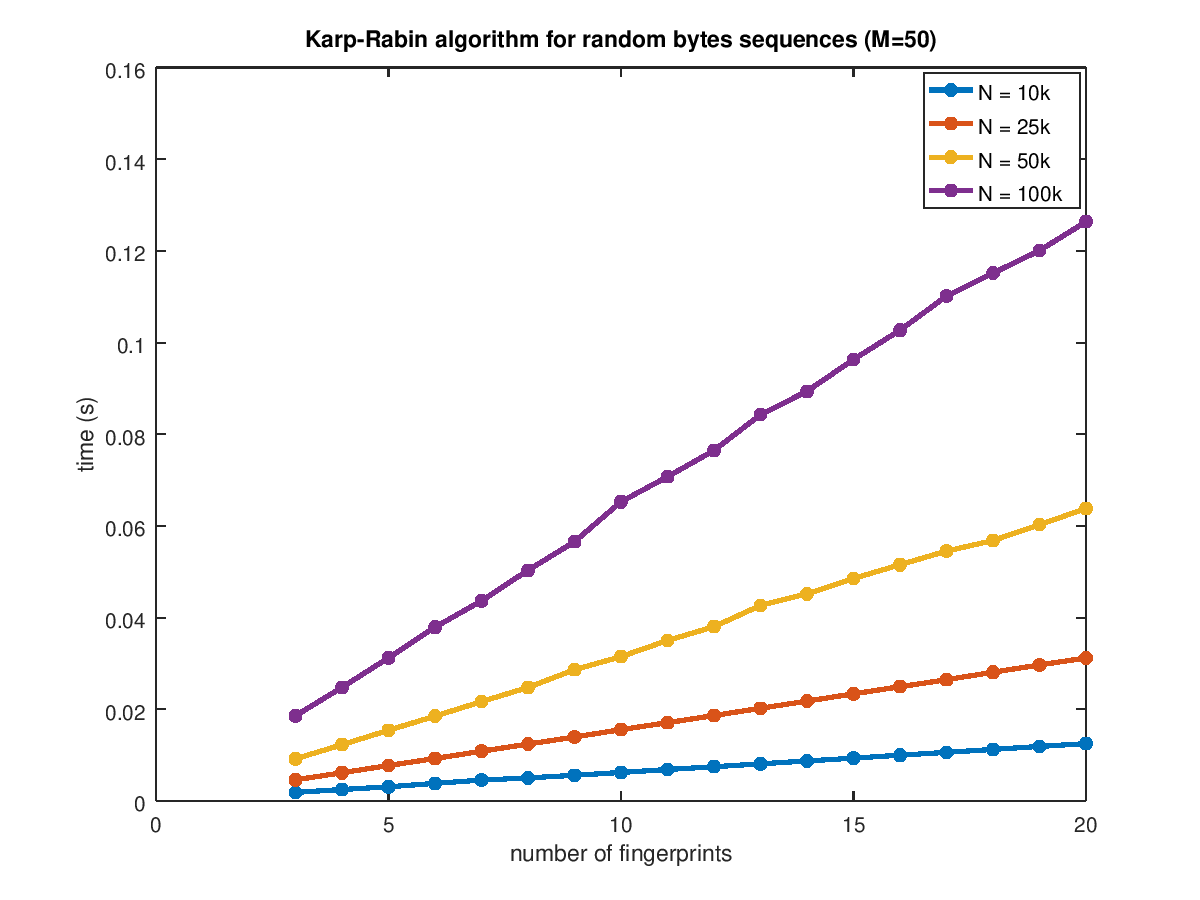
\includegraphics[width=\linewidth]{karp2.png}
    \caption{Average time comparison for different k and pattern lengths.}
  \end{subfigure}
  \caption{Karp-Rabin algorithm experiments.}
  \label{fig:karp}
\end{figure}

Let $s_t$ and $s_p$ be respectively the text string and the pattern string. Let $n = |s_t|, m = |s_p|$. Suppose $k$ fingerprint functions are employed. Then we want to prove that:

$$T(n, m) = \mathcal{O}(m + n)$$
$$S(n, m) = \mathcal{O}(1)$$

The spatial complexity is trivially the storage required to store the pre-computed fingerprints for each alphabet character, which is clearly constant w.r.t. the input $n, m$.

If we assume that the fingerprints tables are pre-computed, the time complexity is merely a result of computing the fingerprint for two character sequences of length $m$, the pattern and the text prefix $s_t[0 ... m]$, and shifting the latter by $n - m$ characters. This must be done $k$ times, one for each fingerprint function. Therefore the time complexity is:

$$T(n, m, k) = \mathcal{O}(k (m + m + (n - m)))$$

However if we assume $k$ to be a constant of the algorithm, the time complexity is simply proportional to the length of the pattern and the text.

\section{Galil-Seiferas algorithm}

\subsection{Description}
The Galil-Seiferas algorithm is a determinstic string-search algorithm with linear time complexity and constant space complexity.

The algorithm is based on the concept of prefix period. Conceptually we say that a string has a period of value $p$ if a second copy of the string shifted by $p$ characters matches the original string in the overlapping parts. We also define the function $reach(p)$ as the maximum value $q$ such that $q = np$ for some $n > 0$, $p$ period of the string. A prefix period is a basic period such that $reach(p) >= kp$ for some constant $k > 0$.

The pre-processing step consists in finding a perfect factorization of the pattern $s_p = uv$ such that $v = z^lz'az'', l >= k$ and $|u| = period(v)$.

Then the text is scanned for any occurrences of $v$. In case $v$ is found we naively check if the preceding portion of the string matches $u$.

\subsection{Implementation}
The actual search algorithm can be considered a variant of the naive approach. The naive approach uses two indices $(p, q) = (0, 0)$ to compare the pattern $s_p$ with the substring $s_t[p ... p + q]$. If a mismatch occurs at any position $q < m = |s_p|$ the indices are trivially updated:

$$(p, q) \leftarrow (p + 1, 0)$$

The Galil-Seiferas algorithm exploits the knowledge of $v$ to perform a non-trivial update (assume $p_1 = period(v)$:

\begin{equation*}
(p, q) \leftarrow
\left\{\begin{alignedat}{2}
& (p + p_1, q - p_1), && kp_1 \le q \le reach_v(p_1) \\
& (p + max(1, q / k), 0), && otherwise
\end{alignedat}\right.             
\end{equation*}

This allows us to perform the search in linear time and with constant space complexity.

\subsection{Performance evaluation}
Let $s_p$ and $s_t$ be respectively the pattern string and the text string and $m = |s_p|, n = |s_t|$.

It is easy to prove that the spatial complexity is constant w.r.t. to the input. In fact we only need to store the decomposition of the pattern string $s_p = uv$.

To analyze the time complexity we separately consider the pre-processing step and the search step. Assume $k = 4$ to be a constant of the algorithm. The pre-processing time is linear w.r.t. the pattern string length. The search algorithm has a time complexity of $T_{search} = \mathcal{O}(n)$. The overall time complexity of Galil-Seiferas is thus $T(m,n) = \mathcal{O}(m + n)$.

\begin{figure}
    \centering
    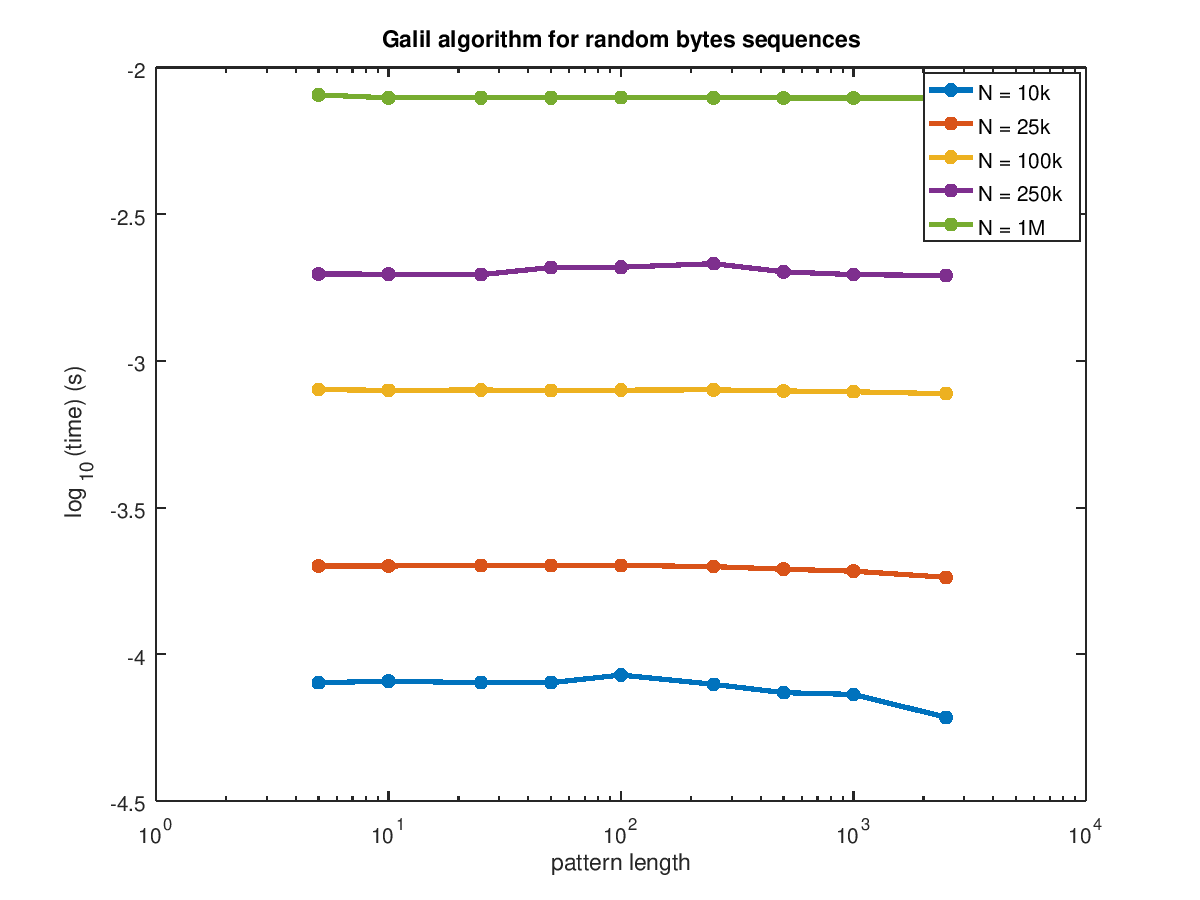
\includegraphics[width=0.5\linewidth]{galil.png}
    \caption{Average time comparison for different text and pattern lengths in Galil-Seiferas algorithm.}
\end{figure}

\end{document}
